\documentclass[12pt,a4paper,xcolor=dvipsnames]{article}

\usepackage[a4paper, top = 2cm, bottom = 2cm, left = 1.5cm, right = 1.5cm]{geometry}
\usepackage[dvipsnames]{xcolor} % Colors

\usepackage{standalone}

\usepackage{setspace}
\usepackage{graphicx}
\usepackage{amsfonts}
\usepackage{amsmath}
%\usepackage{tikz}
\usepackage[dvipsnames]{xcolor}
\usepackage{pdfpages}
\usepackage{epigraph}
\usepackage{csquotes}
\usepackage{natbib}
\usepackage{accents}
\usepackage{pdfpages}

% Bibliography
%\usepackage{xcolor}
\usepackage[dvipsnames]{xcolor}
\usepackage{hyperref}
\hypersetup{
colorlinks=true,
citecolor=MidnightBlue,
linkcolor=MidnightBlue,
pdfpagemode=FullScreen}

\usepackage{listings}
\lstset{frame=tb,
  language=Matlab,
  aboveskip=3mm,
  belowskip=3mm,
  showstringspaces=false,
  columns=flexible,
  basicstyle={\small\ttfamily},
  numbers=none,
  numberstyle=\tiny\color{gray},
  keywordstyle=\color{Red},
  commentstyle=\color{MidnightBlue},
  stringstyle=\color{Red},
  breaklines=true,
  breakatwhitespace=true,
  tabsize=3
}

\usepackage{natbib}
\usepackage[noabbrev]{cleveref}
\setcitestyle{authoryear,open={(},close={)}}
\bibliographystyle{plainnat}


\usepackage{subfiles}

\usepackage{url}
\urlstyle{same} % omit this command if you want monospaced-font look
\newcommand\purl[1]{\protect\url{#1}} % "protected url"

\setlength\parindent{0pt}
\spacing{1.2}

\begin{document}

\begin{center}
       \vspace*{4cm}
       \huge\textbf{Project 6} \\
       \vspace{0.4cm}
       \large \textbf{Public Finance in Macroeconomics} \\
       \vspace{0.5cm}
        \large Handed in by the \textcolor{	RubineRed}{\textbf{Heterogeneous Geeks}} \\
        \vspace{0.3cm}
        a.k.a. Vivien Voigt, Thong Nguyen, 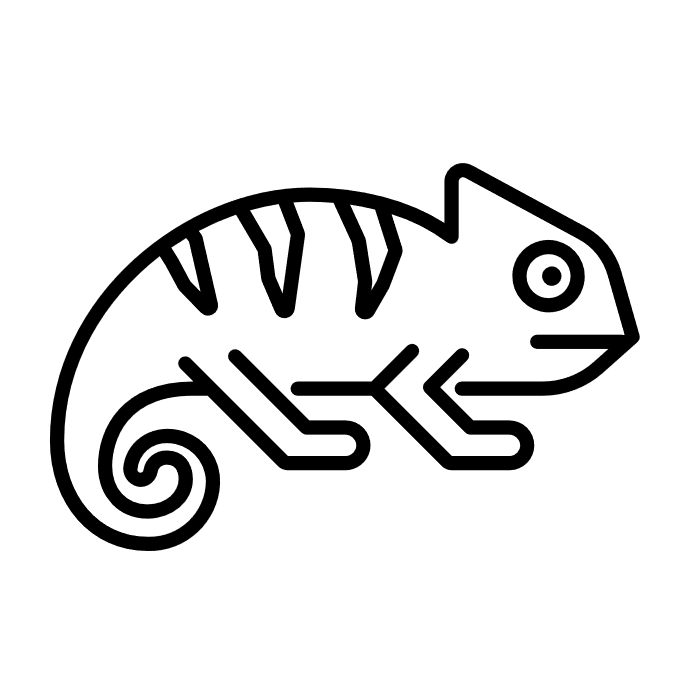
\includegraphics[scale=0.06]{geek.png}\\Davide Difino \& Celina Proffen \\
       \vspace{1.5cm}
       \vfill



        Project in the context of Prof. Ludwig's course: \\
        \textbf{Public Finance in Macroeconomics: Heterogenous Agent Models}\\
        at the Graduate School of Economics, Finance, and Management
       \vspace{0.8cm}
   \end{center}

\newpage
\subsection*{Exercise 1}
Please refer to EX1.m.

\subsubsection*{Exercise 1.2}
An OLG economy might not be Pareto efficient in equilibrium if capital output elasticity ($\alpha$) is low enough. This lead the economy to accumulate more capital than indicated by the "golden rule" that is, the capital stock that maximizes per-capita consumption. The reduction of per-capita consumption level is given by the fact that the return of capital implied by the capital stock is lower than the growth of the economy. Then, if the economy has infinite horizon, it would be always possible to transfer resources from the future, resulting in a Pareto improvement (is this result equivalent to Hilbert's paradox?).  

\subsection*{Exercise 4}
The assigned paper "Education Policy and Intergenerational Transfers in Equilibrium“ develops a heterogenous agents OLG model to assess how financial aid policies act on education, labor and savings decisions of households. It also analyses the welfare effects of policies, concluding that it would be beneficial for society (in this case everything is calibrated to the United States) if more direct financial aid in form of ability-based grants would be handed out to students. 

The agents differ in their “states” and “possible choices” over the life cycle. Young people have to choose their level of education (no high school degree, high school or college) depending on how much education costs in terms of financing and psychic costs. Both are different for agents of different background and with different abilities. In particular, the available loans and grants differ in parents wealth and own abilities; financing options overall are public and private loans, financial aid, their own working activity, in addition to an intra-vivo transfer that students receive from their parents at the beginning of their model life. 

Parents are matched given the man’s and woman’s education and always have two children of the same sex. They care about their children’s direct well-being (altruistic motive) but also directly about their level of education (something like a prestige motive, paternalistic preferences). Their own wealth as well as the financing opportunities of the child determines the inter vivo-transfers they give to their kids. Cognitive and non-cognitive skills are transmitted across generations dependent on parents’ education and skills, and important for the psychic costs of studying (mentioned above) and the labour productivity. 
It is to mention that there are really many levels of heterogeneity amongst agents. Some of them are: Age, gender, initial wealth, cognitive and non-cognitive abilities, education, returns to education and the psychic costs of schooling, … (?)

We want to mention some model features which we found particularly interesting:
\begin{itemize}
    \item There is financial markets and risk that is only partially insurable (uninsureable risk: idiosyncratic income risk, risk of being born into a disadvantaged family, risk of marrying someone who is bad for your income, and shocks affecting the psychic costs of eduction)
    \item Agents work and earn, they have gender specific income trends and can co-insure themselves by accounting for the spousal labor supply too
    \item model earnings as a gender-specific stochastic Roy model with a separate process for each education group and dependent on ability
    \item firm side: the aggregate production function depends on inputs from three types of education and allows for imperfect substitutability between males and females of the same skill
    \item economies of scale in household consumption
    \item debt limits vary over the life cycle
\end{itemize}

The model is calibrated with a wide variety of data sources. Amongst them are “the Current Population Survey (CPS), the Panel Study of Income Dynamics, NLSY79 and NLSY97, the National Center for Education Statistics (NCES), the Survey of Consumer Finances (SCF), and the National Accounts“ (see p. 4 of the paper). 

They estimate the model in various stages, and are very careful to explain most steps specifically (sometimes in the Appendix). After exogenously determining some parameters, the first estimations occur in separate calibrations, and the remaining model parameters are estimated in a General Equilibrium context. 

Finally, there are some policy experiments carried out. \textcolor{red}{I still need to finish this - Celina}


\pagebreak

\end{document}
